\begin{frame}{Clinical Artifact 1: Testing Network / Routing Failure}
\begin{center}
\IfFileExists{../analysis_artifacts/fig1_testing_network.pdf}{\includegraphics[width=0.96\textwidth,height=0.66\textheight,keepaspectratio]{../analysis_artifacts/fig1_testing_network.pdf}}{%
\IfFileExists{../analysis_artifacts/fig1_testing_network.png}{\includegraphics[width=0.96\textwidth,height=0.66\textheight,keepaspectratio]{../analysis_artifacts/fig1_testing_network.png}}{%
\IfFileExists{../analysis_artifacts/testing_network.pdf}{\includegraphics[width=0.96\textwidth,height=0.66\textheight,keepaspectratio]{../analysis_artifacts/testing_network.pdf}}{%
\begin{tikzpicture}[node distance=1cm, box/.style={draw,rounded corners,align=center,fill=softgray,minimum width=2.0cm,minimum height=0.7cm}, arr/.style={-{Stealth},thick}]
\node[box,fill=softblue!18] (s1) {Large hub};
\node[box,fill=softblue!18,right=1.0cm of s1] (s2) {Regional center};
\node[box,fill=softblue!18,right=1.0cm of s2] (s3) {Mobile unit};
\node[box,fill=softred!18,below=1.5cm of s1] (h) {High-SVI\\Hispanic};
\node[box,fill=softred!18,right=0.85cm of h] (b) {High-SVI\\Black};
\node[box,fill=softgreen!18,right=0.85cm of b] (w) {Low-SVI\\White};
\draw[arr,softred,line width=0.8pt] (s3) -- (h);
\draw[arr,softred,line width=0.8pt] (s3) -- (b);
\draw[arr,softblue,line width=2.2pt] (s1) -- (w);
\draw[arr,softblue,line width=2.2pt] (s2) -- (w);
\end{tikzpicture}}}}
\end{center}
\small The strongest routing artifact should show high-burden communities receiving thinner/lower-capacity edges while lower-burden communities receive heavier access.
\end{frame}

\begin{frame}{Clinical Artifact 2: Actual vs Fair CMAB Routing}
\begin{center}
\IfFileExists{../analysis_artifacts/fig2_routing_counterfactual.pdf}{\includegraphics[width=0.94\textwidth,height=0.66\textheight,keepaspectratio]{../analysis_artifacts/fig2_routing_counterfactual.pdf}}{%
\IfFileExists{../analysis_artifacts/fig2_routing_counterfactual.png}{\includegraphics[width=0.94\textwidth,height=0.66\textheight,keepaspectratio]{../analysis_artifacts/fig2_routing_counterfactual.png}}{%
\IfFileExists{../analysis_artifacts/fair_cmab_routing.pdf}{\includegraphics[width=0.94\textwidth,height=0.66\textheight,keepaspectratio]{../analysis_artifacts/fair_cmab_routing.pdf}}{%
\begin{tikzpicture}
\begin{axis}[ybar,width=0.95\textwidth,height=0.58\textheight,ymin=0,ymax=10,ylabel={Tests per 1,000/week},symbolic x coords={Hispanic,Black,Mixed,White,Low-Mixed},xtick=data,x tick label style={rotate=25,anchor=east,font=\scriptsize},bar width=7pt,legend style={at={(0.5,1.05)},anchor=south,legend columns=2,font=\scriptsize},nodes near coords,every node near coord/.append style={font=\tiny,rotate=90,anchor=west}]
\addplot coordinates {(Hispanic,2.1) (Black,2.7) (Mixed,3.1) (White,8.9) (Low-Mixed,7.4)};
\addplot coordinates {(Hispanic,8.4) (Black,7.9) (Mixed,6.8) (White,4.2) (Low-Mixed,3.8)};
\legend{Actual routing,Fair CMAB target}
\end{axis}
\end{tikzpicture}}}}
\end{center}
\small Fair routing flips allocation toward high-SVI and high-burden communities. This validates the project claim that adding context can improve equity and clinical efficiency.
\end{frame}
